\chapter{Diseño}

En esta sección describiremos el diseño de la aplicación, tanto en el aspecto de la estructura de navegación como en el artístico y de interfaz.

\section{Estructura de navegación}

La estructura de navegación que hemos creado para la aplicación es sencilla y no muy extensa, persiguiendo el objetivo de conseguir la mayor facilidad de uso posible. De este modo, se evita un entramado laberíntico que empeora la experiencia de usuario.

En la siguiente figura (\ref{fig:navegacion}) podemos observar distintos elementos. Por una parte, tenemos las cuatro actividades que conforman la aplicación y que se muestran a continuación. A su vez, dentro de casi todas ellas hay fragmentos con distinta funcionalidad e interfaz: 
\begin{itemize}
    \item \textbf{Actividad splash:} Su función es únicamente mostrar una imagen mientras se inicia la aplicación.
    
    \item \textbf{Actividad principal:} Su contenido se alterna entre tres fragmentos distintos. Por una parte, el fragmento de inicio, el cual muestra y permite acceder a las diferentes partes del test SPPB. Por otra, el fragmento de usuarios, que muestra una lista con todos los usuarios guardados y la posibilidad de crear nuevos o borrar existentes. Por último, el fragmento de puntuación (que también es usado en la actividad tests), el cual exhibe la puntuación desglosada del usuario seleccionado.
    
    \item \textbf{Actividad tests:} En ella se muestran los fragmentos de las tres partes del test SPPB, cada uno con su propia funcionalidad. Al finalizar una de las pruebas o todas ellas, también aparece el fragmento de puntuación.
    
    \item \textbf{Actividad instrucciones:} Esta actividad alberga un elemento que ofrece Android denominado ViewPager, el cual permite deslizar la pantalla entre distintas diapositivas de instrucciones.
\end{itemize}

\begin{figure}[H]
	\centering
	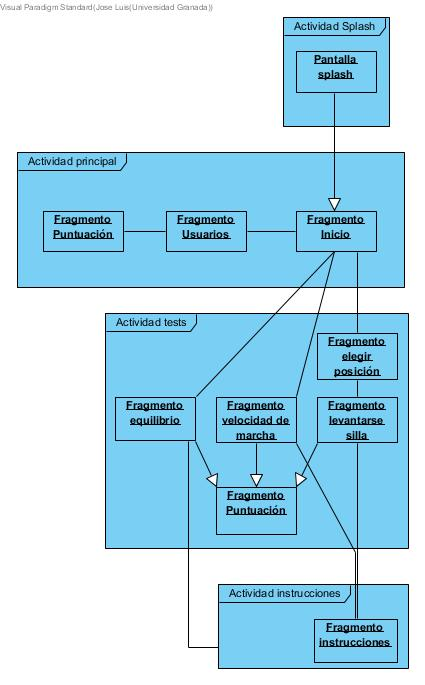
\includegraphics[scale=0.70]{imagenes/pantallas.jpg}
	\caption{Navegación entre pantallas\label{fig:navegacion}}
\end{figure}

\section{Diseño de la base de datos}

En este apartado describiremos el diseño propuesto para la base de datos. Como hemos apuntado anteriormente, las necesidades de almacenamiento serán muy básicas, siendo el objetivo guardar únicamente algunos datos producto de la realización de la prueba SPPB bajo un nombre o seudónimo elegido por el propio usuario.

\begin{figure}[H]
	\centering
	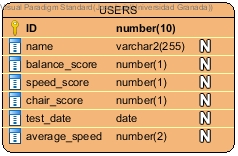
\includegraphics[scale=0.70]{imagenes/USERS.jpg}
	\caption{Diseño de la base de datos\label{fig:base_datos}}
\end{figure}

En la figura superior (\ref{fig:base_datos}) vemos un esquema UML de la base de datos. Podemos apreciar que sólo cuenta con una tabla que se usa tanto para almacenar el nombre como los resultados. El motivo radica en que la aplicación carece de la necesidad de administrar otros datos del usuario, los cuales podrían ser más sensibles y romper con el Reglamento General de Protección de Datos (GDPR). De este modo ahorramos tener que crear una tabla distinta destinada a guardar otros datos de identidad del usuario como podrían ser apellidos, edad o correo electrónico.

La única tabla, de nombre \textit{USERS}, cuenta con un total de 7 columnas. A parte de ID, usada para identificar mediante un número único a cada usuario, encontramos las siguientes:
\begin{itemize}
    \item \textbf{name:} De tipo texto, guarda el nombre o seudónimo introducido por el propio usuario para identificar la información de manera más sencilla.
    
    \item \textbf{balance\_score, speed\_score y chair\_score:} Todos de tipo numérico, ofrecen la posibilidad de registrar el resultado individual en las tres pruebas del test SPPB. Guardar dichos resultados individualmente garantiza la posibilidad de actualizar una prueba concreta a posteriori.
    
    \item \textbf{test\_date:} De tipo fecha, su objetivo es guardar en qué día se ha llevado a cabo el último test realizado. Aún no tiene uso, se guarda con vistas a añadir una funcionalidad futura.
    
    \item \textbf{average\_speed:} De tipo numérico, guarda la velocidad media calculada a raíz de la prueba de velocidad de marcha.
\end{itemize}

\section{Diseño de la interfaz}

El diseño de la interfaz ha sido una de las partes más importantes del desarrollo. Son muchas las razones que podemos dar e infinitos los artículos en internet que insisten encarecidamente en los beneficios de tomárselo en serio. Algunas razones listadas en el blog \textit{International Hispanic Community} \cite{design} son:
\begin{itemize}
    \item Hace que tu producto marque la diferencia.
    \item Da seriedad.
    \item Facilita la vida del usuario.
    \item Puede hacerte triunfar respecto a otras opciones.
\end{itemize}

Por todo ello, hemos preferido no mantener el diseño por defecto con el que cuentan los distintos elementos de la interfaz, dando un aspecto mucho más actual y con una mayor personalidad.

Es importante recalcar que tanto el diseño de la interfaz como el de las distintas imágenes se ha llevado a cabo sin ninguna noción de estilo, puesto que no es un ámbito que se imparta en el área de la programación. Por tanto, es muy probable que sean muchos los elementos que incumplan propiedades importantes dentro de la estructuración visual y gráfica que tendría que tener una interfaz, aunque se ha intentado conseguir un resultado profesional.


\subsection{Colores utilizados}

El color elegido como principal ha sido el azul (\#2196F3). Este se ha utilizado de forma recurrente en diferentes componentes como botones, textos y fondos. 

Por otra parte y con el objetivo de hacer más fácil de entender y recordar cada test mediante la asociación del mismo a un color, se ha decidido establecer una tonalidad diferente para cada una de las pruebas individuales. Finalmente, tras buscar combinaciones que resultasen agradables y fuesen suficientemente desiguales entre ellas, hemos optado por asignar una gama verde a la prueba de equilibrio (\#4CAF50), morada índigo a la prueba de velocidad de marcha (\#7C4DFF) y naranja al de levantarse de la silla (\#E64A19).

\subsection{Bocetos iniciales}

A la hora de determinar la apariencia y estructura gráfica de la aplicación, el primer paso no podía ser otro que un boceto hecho a mano alzada. Al realizarlo, obtenemos una primera impresión de cómo de bien o mal integrados estarían cada uno de los elementos. Además, al poder llevarse a cabo y modificarse de forma rápida y sencilla, es muy útil para mostrarlo a otras personas y obtener unas primeras opiniones que ayuden a modificar y mejorar el aspecto a lápiz, lo cual es mucho más efectivo que hacerlo más tarde sobre la interfaz real.

Puesto que la aplicación, al menos de momento, no tendrá demasiados apartados, ha sido relativamente fácil diseñar todas las pantallas que serán visibles al usuario. En total se trata de cuatro pantallas con diseños distintos. Habrá varios apartados que reutilicen los mismos diseños, como por ejemplo las pantallas visibles durante la ejecución de los tests. La estructura será la misma en todas ellas, pero cada una tendrá imágenes y color diferentes.

\begin{figure}[H]
	\centering
	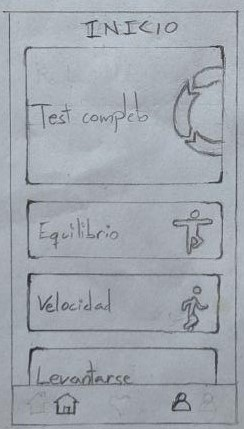
\includegraphics[scale=1]{imagenes/boceto_inicio.jpg}
	\caption{Boceto a lápiz de la pantalla de inicio\label{fig:boceto_inicio}}
\end{figure}

En la figura \ref{fig:boceto_inicio} podemos ver la idea inicial sobre cómo estructurar la \textbf{pantalla de inicio}. Cuenta con un título indicativo que reza \textit{INICIO}, útil para que el usuario sepa en qué pantalla se encuentra. Tras él, podemos ver cuatro botones, tres de ellos correspondientes a cada una de las pruebas que componen el test SPPB. Hay un cuarto botón, que en el boceto destaca más por su tamaño, el cual permite realizar el test completo (las tres pruebas que componen SPPB de forma seguida).

Por último se observa un menú inferior con únicamente dos opciones, la primera con un icono de una casa, para la pantalla Inicio, y la segunda con el icono de una persona, para la pantalla Usuarios.

\begin{figure}[H]
	\centering
	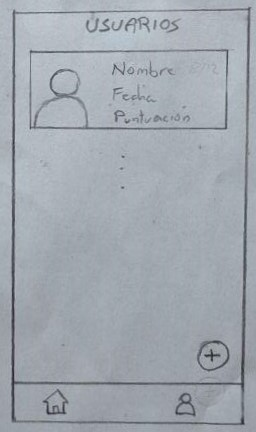
\includegraphics[scale=1]{imagenes/boceto_usuarios.jpg}
	\caption{Boceto a lápiz de la pantalla de usuarios\label{fig:boceto_usuarios}}
\end{figure}

Lo que puede observarse en la figura superior (\ref{fig:boceto_usuarios}) es la \textbf{pantalla de usuarios}. Como se puede comprobar, a parte del título hay una lista que pretende mostrar todos los usuarios guardados. Cada uno de los elementos muestra un nombre, una fecha de realización del test y una puntuación. No obstante, estos elementos se reducirán a uno sólo en la implementación, el del nombre, con el objetivo de que el texto pueda verse más grande y de que no se desfigure si las preferencias de tamaño de texto establecidas por el usuario son demasiado grandes. Así, facilitamos la accesibilidad al mejorar su optimización para personas con problemas de vista.

Por otra parte también se puede ver un icono de usuario, el cual también se modificará en la versión implementada, sustituyéndolo por un número con la puntuación obtenida. Este número adquirirá un color distinto dependiendo del rango de limitación en el que se encuentre, pasando desde rojo (en el peor caso), a naranja (limitación moderada), amarillo (limitación leve) y por último, verde (limitación mínima).

\begin{figure}[H]
	\centering
	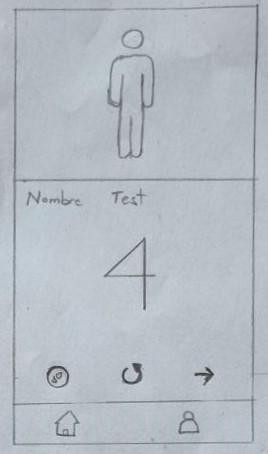
\includegraphics[scale=1]{imagenes/boceto_test.jpg}
	\caption{Boceto a lápiz de la pantalla de test\label{fig:boceto_test}}
\end{figure}

En esta imagen (figura \ref{fig:boceto_test}) se observa la que será la pantalla de ejecución del test. Se encuentra divida en aproximadamente dos mitades. La primera de ellas cuenta con una imagen en la que se mostrará un dibujo con la posición que se debe adoptar. Esta imagen se actualizará en caso de perder el equilibrio, de estar sentado o levantado, o de estar caminando o parado, añadiendo una mejor apariencia y un mayor dinamismo.

La otra mitad será la que albergue los controles y la información de ejecución. A parte del nombre del test actual, mostrará un botón de inicio (play) hasta el momento en el que sea pulsado. Posteriormente y a medida que se realiza el test, actualizará contadores como el cronómetro o el número de veces que se ha repetido el movimiento. Además, habrá botones para silenciar el sonido, para acceder a la información y para repetir la prueba o indicar incapacidad para realizarla.

\begin{figure}[H]
	\centering
	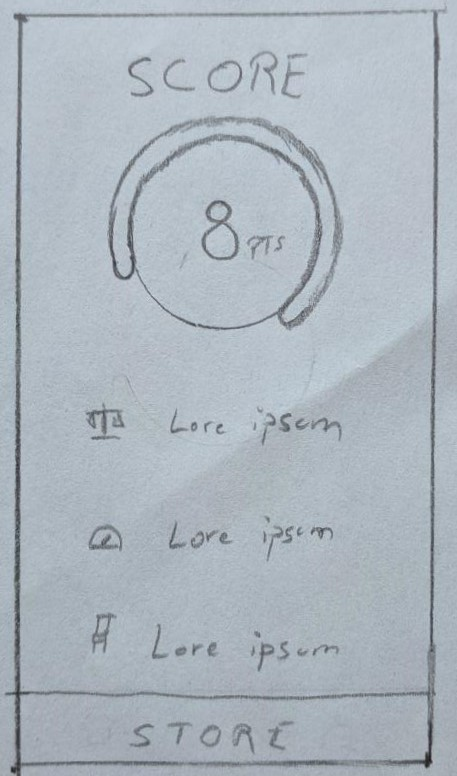
\includegraphics[scale=0.55]{imagenes/boceto_score.jpg}
	\caption{Boceto a lápiz de la pantalla de puntuación\label{fig:boceto_puntuacion}}
\end{figure}

Por último, en la figura \ref{fig:boceto_puntuacion} vemos lo que es una primera aproximación a la pantalla de puntuación. Esta pantalla será mostrada cuando pulsamos en algún usuario de la lista de usuarios o al finalizar un test, como vimos en el esquema de navegación entre pantallas de la figura \ref{fig:navegacion}. 

En ella mostraremos un círculo con progresión que estará más o menos relleno según la cantidad de puntos obtenida (entre 0 y 12). Posteriormente, se mostrará de forma individual el número de puntos alcanzados en cada uno de los tests. En caso de haber realizado una única prueba, se ocultarán los nombres e iconos de las no realizadas. Por último, también se podrá ver un botón de \textit{guardar} (STORE), mostrado únicamente si había un usuario seleccionado.

Esta vista también sufrirá cambios en la implementación, entre ellos la eliminación del título, la incorporación de un nuevo campo en el que se muestre el cálculo de velocidad media de marcha, o la sustitución de los iconos por un rectángulo pequeño con el color de cada prueba y el nombre.

\subsection{Imágenes utilizadas}

Como se indicó en el requisito no funcional número cinco (\ref{RNF:5}), es importante no usar imágenes o iconos con derechos de autor. No obstante, si queremos conseguir una apariencia con un estilo cohesionado y uniforme, la tarea se complica enormemente si pretendemos utilizar únicamente imágenes conseguidas de internet. Por ejemplo, es poco probable encontrar iconos que representen las tres partes del test SPPB con un diseño similar, y más improbable se vuelve aún hallar recursos gráficos parecidos de una silueta humana en las posiciones que requiere el test (tándem, sentado, andando, pérdida del equilibrio, etc).

Ante este problema, se tomó la decisión de realizar de forma personal toda la iconografía y diseños. Para tal fin, se utilizó una herramienta de diseño vectorial. Las imágenes vectoriales tienen la característica de no estar formadas por conjuntos de píxeles sino por formas geométricas y fórmulas matemáticas, las cuales permiten que la imagen nunca pierda calidad independientemente del tamaño con el que se redimensione. La gran ventaja que obtenemos es que, a parte de tener un tamaño mucho menor que las imágenes convencionales, no hay que preocuparse de cómo de grande es la pantalla del dispositivo en el que se muestre, puesto que siempre se visualizará con la máxima calidad posible\cite{vectorial}.

\subsubsection{Logotipo}

\begin{figure}[H]
	\centering
	
\includegraphics[scale=0.5]{imagenes/icon_small.png}
	\caption{Logotipo de la aplicación\label{fig:logo}}
\end{figure}

Dicho esto, comencemos mostrando y comentando el logotipo que se puede ver en la anterior figura (\ref{fig:logo}). Es un logotipo que busca ser simple pero mostrar a la vez la esencia de la aplicación. Se ha elegido darle forma de corazón por la relación del test SPPB con la detección de fragilidad en ancianos (capítulo \ref{ch:descripcion}) y las implicaciones en la salud que esto tiene. Además, se ha coloreado con los tres pigmentos establecidos para cada una de las partes del test, de forma que se resuma el estilo de la aplicación desde incluso antes de acceder a ella.

\subsubsection{Figuras de ejemplo}

\begin{figure}[H]
	\centering
	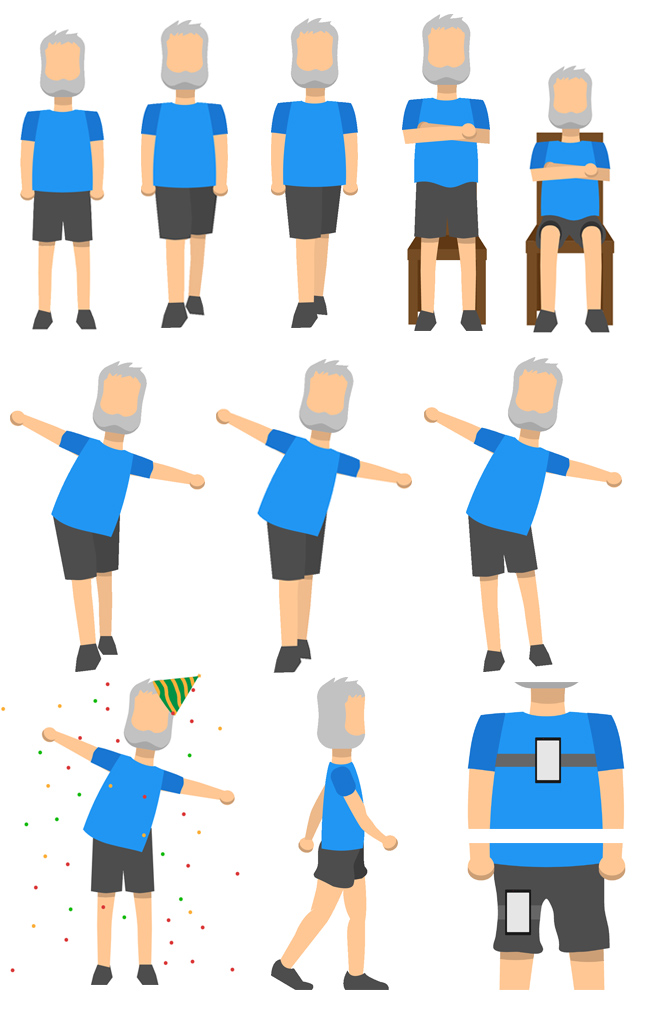
\includegraphics[scale=0.43]{imagenes/figuras_ejemplo.jpg}
	\caption{Todas las figuras de ejemplo para SPPB\label{fig:figuras_ejemplo}}
\end{figure}

En la imagen superior (\ref{fig:figuras_ejemplo}) podemos ver el personaje diseñado con el objetivo de mostrar la posición del test en cada momento, así como otra información relevante. Se trata de un diseño simple, sin apenas rasgos faciales ni de vestimenta para intentar convertirlo en lo más polivalente posible. 

Para diseñarlo nos hemos basado en un tutorial creado por Arumadigital \cite{Arumadigital} y en los personajes del programa de Mikel Izquierdo \cite{SPPB_clasificacion}, con el que hemos dado forma al primer personaje (arriba a la izquierda). Posteriormente, modificamos distintas partes y posturas hasta conseguir una variante del personaje que se adaptase a cada una de las posiciones necesarias.

\subsubsection{Iconos de los tests}

\begin{figure}[H]
	\centering
	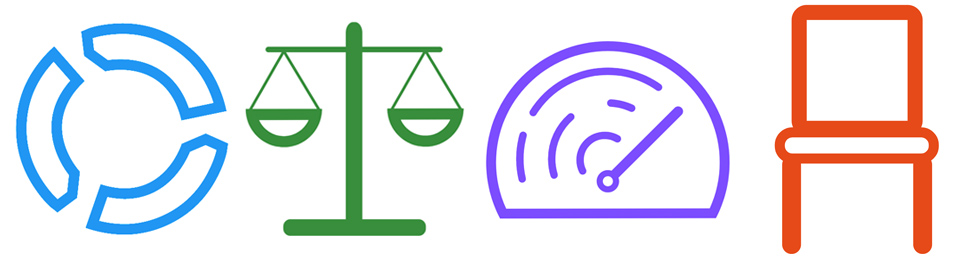
\includegraphics[scale=0.35]{imagenes/iconos.jpg}
	\caption{Todas los iconos de los tests SPPB\label{fig:todos_iconos}}
\end{figure}

En la figura \ref{fig:todos_iconos} vemos los cuatro iconos que aparecerán en cada uno de los botones que llevan a los distintos tests en la pantalla de inicio. Se ha intentado que tengan un estilo similar al estar formados por líneas y ningún relleno.

Aquí aparecen coloreados con su gama correspondiente, aunque en los botones de la pantalla de inicio serán blancos. Estos botones coloreados se usarán en otros elementos como los \textit{``Atajos''} de Android, que permiten acceder a una parte concreta de la aplicación desde fuera de la misma.

\newpage
\subsubsection{Imágenes varias}

\begin{figure}[H]
	\centering
	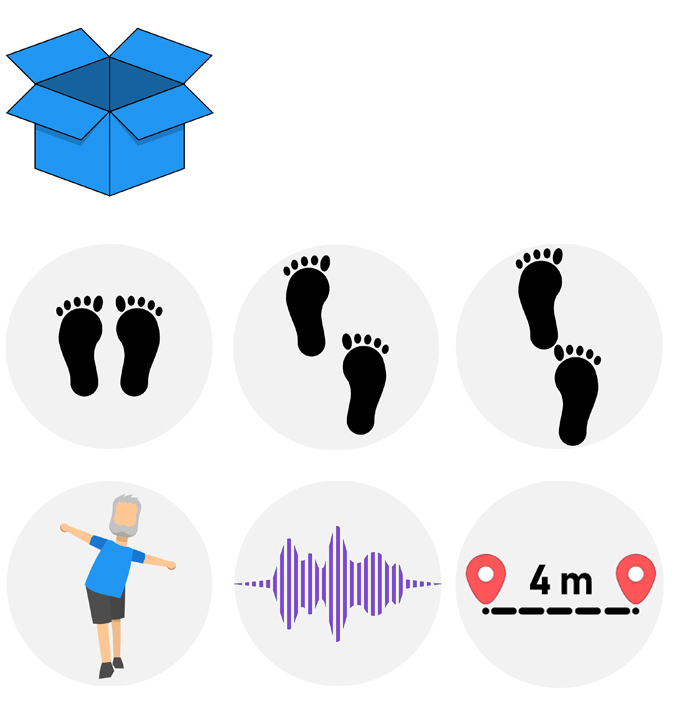
\includegraphics[scale=0.45]{imagenes/slides.jpg}
	\caption{Imágenes de instrucciones y miscelánea\label{fig:instrucciones}}
\end{figure}

Por último, en la figura \ref{fig:instrucciones} vemos siete dibujos más. El primero, la caja situada en primera fila, se utiliza para ilustrar gráficamente la pantalla de \textit{Usuarios} cuando no hay ningún usuario (valga la redundancia) almacenado. Al estar abierta y vacía, simboliza ausencia de elementos. Para realizarla nos basamos en un tutorial creado por The Simple Designers \cite{SimpleDesigners}.

En las dos siguientes filas se aprecian círculos que contienen distintas figuras de plantas del pie, sonido, distancia, etc. Han sido creadas con el objetivo de ser utilizadas en las diapositivas que pueden verse en la actividad de instrucciones. Hay varias imágenes de instrucciones que no aparecen aquí ya que para crearlas hemos reutilizado otras como las figuras de ejemplo \ref{fig:figuras_ejemplo}.

\subsection{Resultado final de la interfaz}

A continuación veremos el resultado final del diseño. Aquí sí podrán apreciarse la aplicación de colores y la integración de imágenes, cosa que en los bocetos a mano alzada no se conseguía. 

\begin{figure}[H]
	\centering
	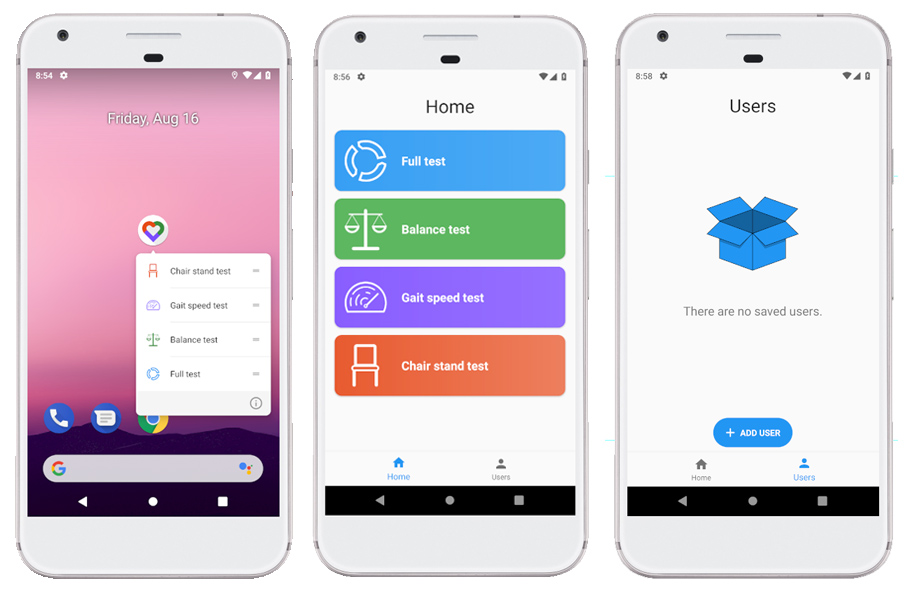
\includegraphics[scale=0.4]{imagenes/capturas1.jpg}
	\caption{Pantallas principales de la aplicación\label{fig:capturas1}}
\end{figure}

En la figura superior (\ref{fig:capturas1}) se observan tres pantallazos. En el primero de ellos aparece el acceso directo a la aplicación, que se muestra con el logotipo del corazón. Si nos fijamos, hay un menú desplegado que cuelga del icono de la app. Este menú cuenta con cuatro de los denominados \textit{atajos} de Android que mencionamos anteriormente y que permiten acceder a cualquiera de las tres pruebas de forma directa, o a la ejecución completa del test SPPB. Se trata de funcionalidades sin demasiada importancia pero que pueden ser útiles en un determinado momento.

En segundo lugar vemos la que finalmente es la \textbf{pantalla principal} de la aplicación. En ella hay cuatro botones con un ligero degradado como ya se adelantó en el boceto, aunque el tamaño y la forma de todos ellos no es igual que en la idea original.

Por último encontramos la \textbf{pantalla de usuarios}. Al no haber ningún usuario guardado, se muestra el dibujo por defecto de la caja vacía junto a un texto explicativo. También hay en esta pantalla un botón azul (el color principal de la aplicación) para añadir usuarios. Ese botón se oculta en caso de que haya una lista superior al tamaño de la pantalla y se realice un desplazamiento o \textit{scrolling} hacia abajo, para volver a mostrarse cuando se realiza hacia arriba.

\begin{figure}[H]
	\centering
	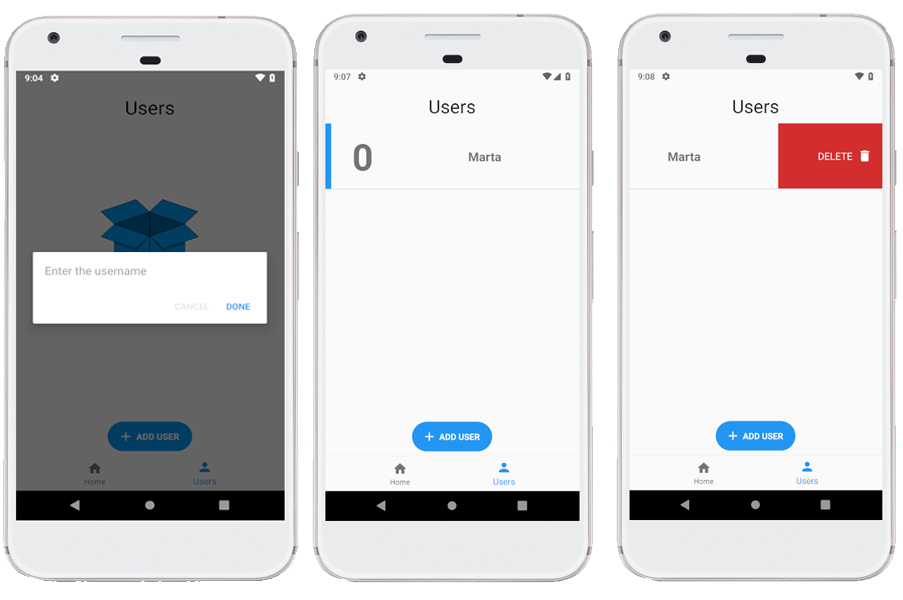
\includegraphics[scale=0.4]{imagenes/capturas_usuarios.jpg}
	\caption{Pantallas de usuarios\label{fig:capturas_usuarios}}
\end{figure}

En la figura \ref{fig:capturas_usuarios} se aprecian más comportamientos de la misma. Por una parte y en primer lugar, tenemos una captura (la situada en la izquierda) en la que se ve un cuadro de diálogo que se muestra al tocar el botón azul de añadir usuarios y que permite realizar lo propio.

En segundo lugar, una vez almacenado el primer usuario, se ve cómo desaparece la caja y texto explicativo por defecto y aparece una fila con un cero (la puntuación actual en los tests) y un nombre de usuario introducido anteriormente. Si nos fijamos, vemos además una línea vertical azul que aparece por defecto y que puede quitarse o volver a ponerse mediante una pulsación larga. Esta línea indica que el usuario se encuentra seleccionado, con lo que al realizar el test nos dará la opción de guardar la puntuación en este usuario.

En la última captura (la más a la derecha) se ve la posibilidad de borrar un determinado usuario mediante un gesto de arrastre. Si dicho gesto se lleva a término, aparecerá un cuadro de diálogo que nos pedirá confirmación antes de eliminarlo completamente, de forma que se eviten quitar algún usuario de forma inintencionada. Esto es importante ya que al almacenarse todos los datos de forma local únicamente, sería imposible recuperar esta información.

\begin{figure}[H]
	\centering
	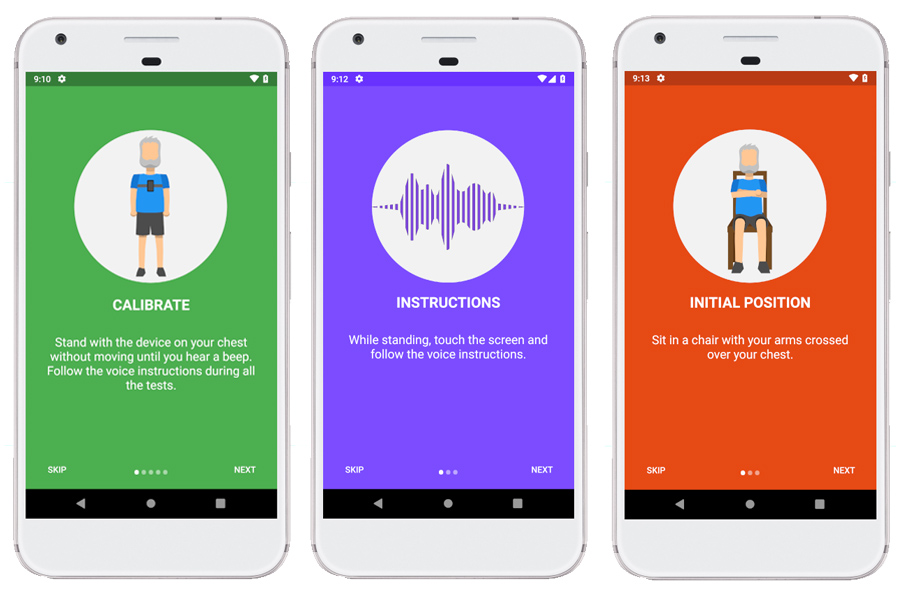
\includegraphics[scale=0.4]{imagenes/capturas_instrucciones.jpg}
	\caption{Pantallas de instrucciones\label{fig:capturas_instrucciones}}
\end{figure}

En este caso, en la figura \ref{fig:capturas_instrucciones} vemos un ejemplo de cómo son las pantallas de instrucciones de cada uno de los distintos tests.

La principal característica común y que a la misma vez sirve para diferenciarlos es el color de fondo. Las instrucciones de la primera captura pertenecerían pues al test de equilibrio, la de la segunda captura al de velocidad de marcha y las de la tercera, al test de levantarse y sentarse cinco veces en una silla. Además, todas ellas tienen un tono más oscuro de ese mismo color para la barra de estado (efecto que hay que programar y que en ningún caso viene por defecto). 

También vemos en todas una imagen, un título y una descripción. Es posible deslizar el dedo a izquierda o derecha para avanzar por las instrucciones. En la parte inferior se observan dos botones y unos puntos que sirven para indicar cuantas diapositivas quedan por ver y cuantas se han visto ya. Además, estos botones que hemos mencionado también permiten navegar entre ellas, moviéndonos de una en una a la siguiente o la anterior, finalizar cuando nos encontramos en la última diapositiva o saltarnos las instrucciones si lo deseamos cuando estamos en la primera.

La actividad de instrucciones aparece de forma automática si es la primera vez que se abre un determinado test tras descargar la aplicación. Posteriormente, pueden consultarse de nuevo todas las veces que haga falta pulsando el botón de información que aparece en las primeras capturas de la figura \ref{fig:capturas_test}.

\begin{figure}[H]
	\centering
	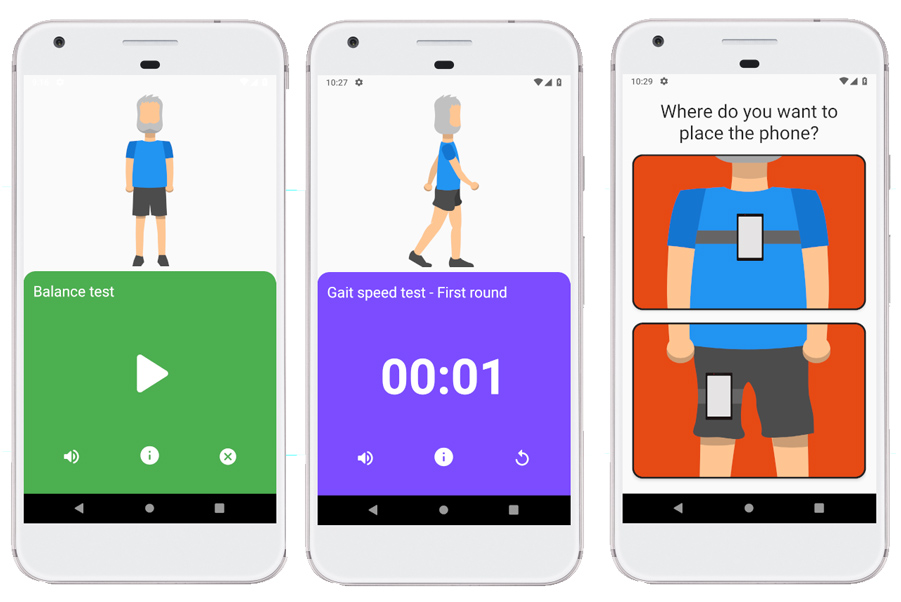
\includegraphics[scale=0.4]{imagenes/capturas_test.jpg}
	\caption{Pantallas de test\label{fig:capturas_test}}
\end{figure}

En la figura \ref{fig:capturas_test} vemos de nuevo tres capturas, correspondientes en este caso a la pantalla de realización de los tests.

Al igual que ocurría en las instrucciones, la mitad inferior que contiene los controles y la información del test establece el color de fondo según qué prueba se está realizando, pudiendo variar entre verde, morado índigo y naranja. La mitad superior alberga una imagen de ejemplo como ya diseñamos en los bocetos a mano alzada, imagen que cambia y se adapta según la parte del test en el que estemos. Por ejemplo, en la prueba de velocidad de marcha se observa como la figura se encuentra en posición de caminar, figura que cambia cuando el usuario deja de realizar el movimiento. 

En la mitad inferior vemos el título de la prueba (e información extra como la posición de los pies que toca en cada momento o la repetición actual del test de marcha), y cuatro controles. El primero es un botón de iniciar (play) que desaparece al clicarlo, y los otros tres son por este orden: silenciar las instrucciones, información y repetir la prueba/incapacidad para realizar la prueba.

En la tercera imagen se aprecia un diseño distinto. Esto se produce únicamente como paso previo al test de silla, el cual sí tiene un diseño similar al de las dos pruebas anteriores. Lo que se hace en esa pantalla es preguntar al usuario el lugar donde querrá colocar el dispositivo, pudiendo elegir entre el pecho y el muslo. Las razones por las que añadimos esta capacidad de elección se explicarán posteriormente y tienen que ver con la fiabilidad de medición del acelerómetro.

\begin{figure}[H]
	\centering
	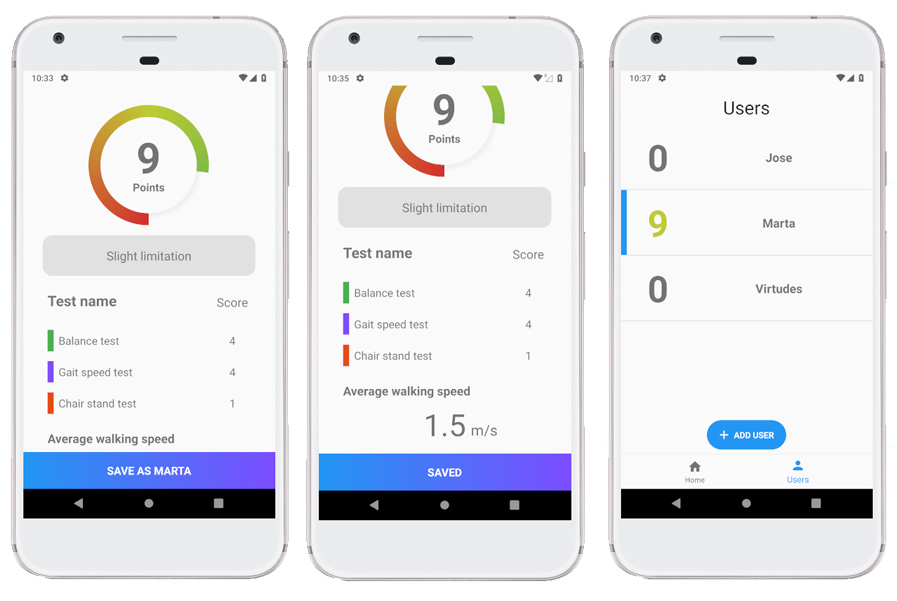
\includegraphics[scale=0.4]{imagenes/capturas_puntuacion.jpg}
	\caption{Pantallas de puntuación\label{fig:capturas_puntuacion}}
\end{figure}

En último lugar comentaremos la figura \ref{fig:capturas_puntuacion}. Es muy similar al diseño realizado en el boceto, salvo pequeños cambios. Esta pantalla aparece tras finalizar alguno de los tests, los tres test o al pulsar uno de los usuarios almacenados de la lista.

En primer lugar contiene un círculo en el que se muestra la puntuación total obtenida y la progresión que supone respecto al total alcanzable. Debajo hay un cuadro con una etiqueta que informa del grado de limitación al que equivale la puntuación conseguida, pudiendo variar desde \textit{limitación grave} en el peor de los casos a \textit{limitación mínima} en el mejor.

Si continuamos descendiendo, encontramos un desglose por pruebas de la puntuación de cada una. Más abajo, si desplazamos la pantalla, aparece la velocidad media de marcha, calculada a raíz de la prueba de velocidad de marcha. Este indicador puede ser muy útil en cuanto a significado clínico.

En último lugar encontramos un botón que aparece en caso de tener un usuario seleccionado antes de iniciar el test. Dicho botón nos ofrece la posibilidad de almacenar el resultado en tal usuario, de forma que la puntuación se mostrará actualizada en la lista, y se nos permitirá acceder en cualquier momento para consultar el desglose de la última ejecución del test.